\clearpage
\begingroup
% Excepción local A3: el diagrama conserva al menos 9 pt en el PDF final.
% newgeometry cambia el área de composición; LuaTeX fija el papel de esta hoja.
\newgeometry{layoutwidth=420mm,layoutheight=297mm,layoutoffset={0mm,0mm},margin=20mm,headheight=27pt,headsep=16pt,includefoot,footskip=28pt}
\setlength{\paperwidth}{420mm}
\setlength{\paperheight}{297mm}
\pagewidth=\paperwidth
\pageheight=\paperheight
\setlength{\headwidth}{\textwidth}
\centering
\begin{minipage}{1000bp}
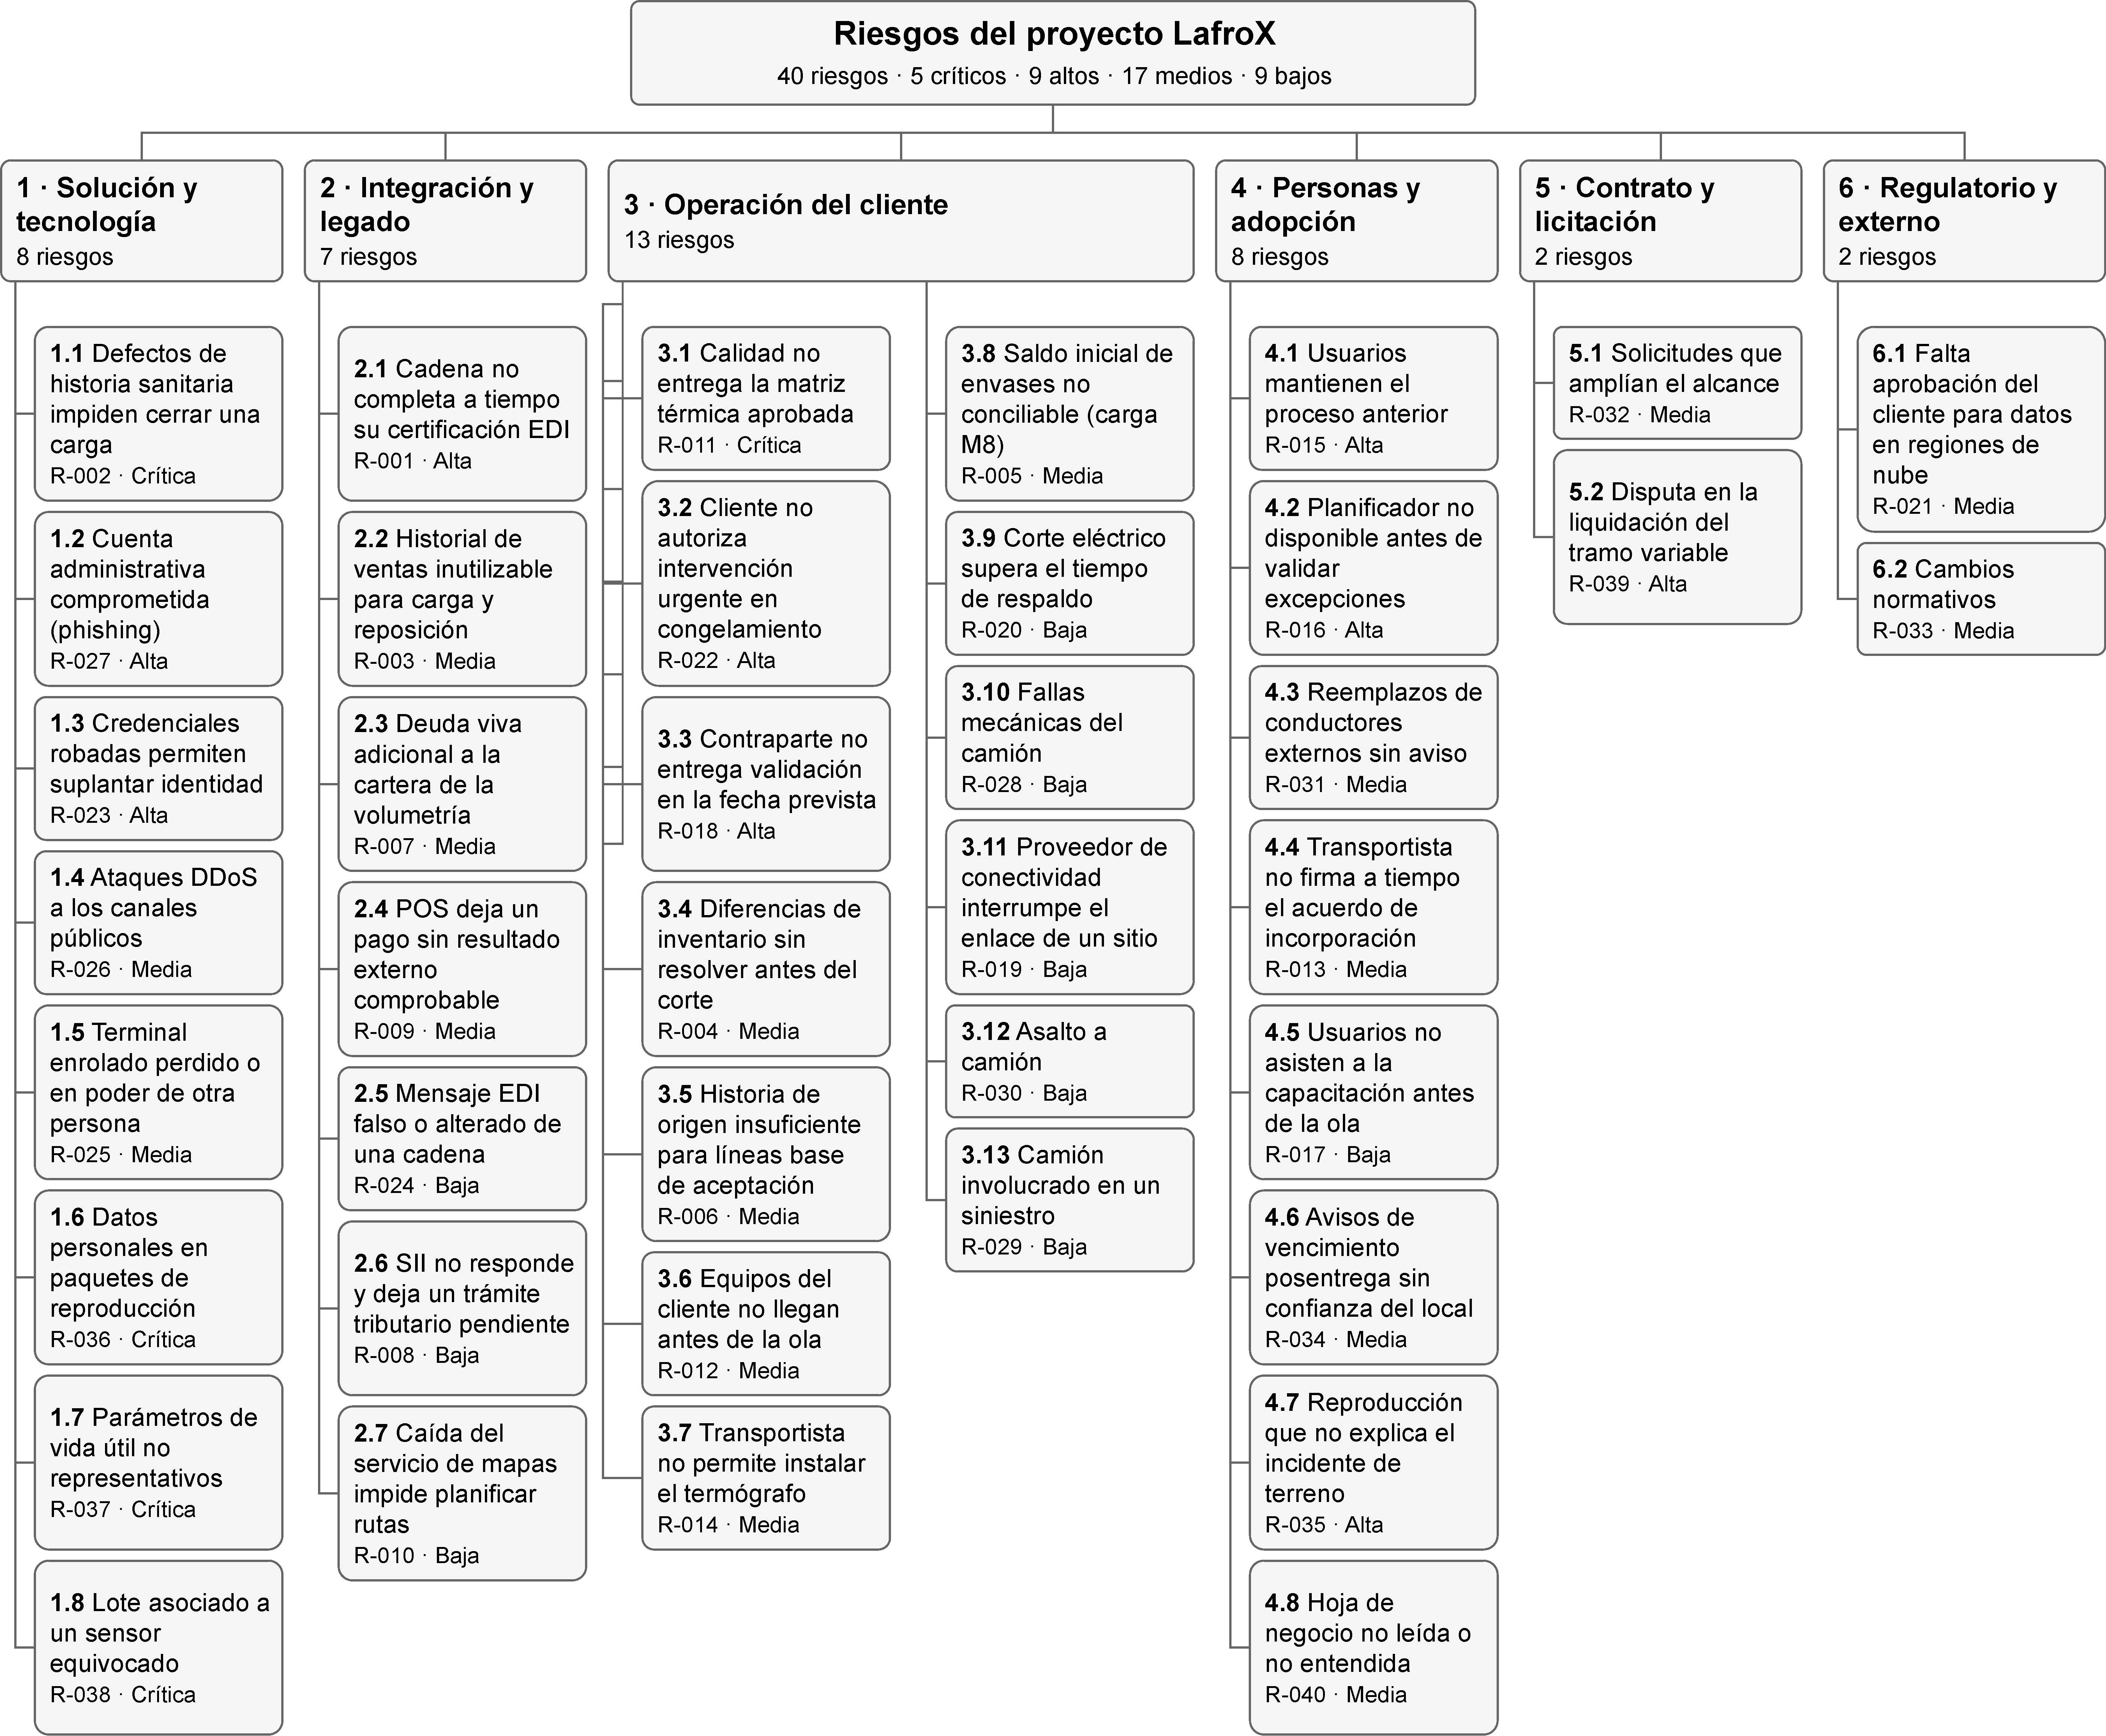
\includegraphics[width=\linewidth,height=0.95\textheight,keepaspectratio]{LafroX_RBS_riesgos.pdf}
{\captionsetup{hypcap=false,skip=6pt}
\captionof{figure}{Estructura de desglose de riesgos (EDR/RBS) del proyecto LafroX: 40 riesgos. Fuente: elaboración propia.}
\label{fig:sd8-rbs}}
\end{minipage}\par
\restoregeometry
\endgroup
\pagewidth=\paperwidth
\pageheight=\paperheight
